\documentclass[12pt, a4paper]{report} 
\usepackage[english]{babel}
\usepackage[utf8]{inputenc}
\usepackage[T1]{fontenc}
\usepackage{geometry}
\usepackage[onehalfspacing]{setspace}
\usepackage{titlesec}
\usepackage{graphicx}
\usepackage{float}
\usepackage{amsmath}
\usepackage{chngcntr}
\usepackage{subcaption}
\usepackage{fancyhdr}
\usepackage{textcomp}
\usepackage[numbers]{natbib}
\bibliographystyle{plain}
\parindent0cm

\title{Transcriptome Analysis of Cladophialophora immunda}
\author{Christina Kustor}
\date{August,2015}


\begin{document}
	\pagenumbering{gobble}
\newpage
\begin{center}
\large {University of Natural Resources and Life Sciences Vienna\\

\includegraphics{pics/boku_logo}\\
\bigskip
\textbf{Department of Biotechnology\\
Extremophile Center}}\\
\vspace*{1,5cm}
\LARGE\textbf{Transcriptome Analysis of 
\textit{Cladophialophora immunda}}\\
\vspace*{0,5cm}
\large {Masterthesis\\
\vspace*{1,5cm}
submitted by\\
Christina Kustor, BSc.\\
Vienna, 2015\\
\vspace*{1cm}
Supervisor: Katja Sterflinger-Gleixner, Assoc. Prof. Dr.\\
Co-Supervisor: Hakim Tafer, Dr.\\}
\end{center}

\newpage
\section*{Acknowledgement}
\newpage
\pagenumbering{arabic}
\section*{Abstract}
The black yeast \textit{Cladophialophora immunda} is known for the capability to grow on polyaromatic hydrocarbons and moreover for the ability to degrate hydrocarbons. \\
The thesis will exermine the way in which the transcriptomes of \textit{Cladophilaphora immunda} can be determined and which genes are transcribed under different conditions. The transcriptome data were obtained with RNA-seq and the analysis were realised with bioinformatics methods. \\
A workflow system for genome annotation with RNA-seq data was developed and followed by performing statistics to obtain a list of genes and their expression level differences between two groups. Furthermore functional annotation and additonal enrichment analysis were performed.\\
....
\\
\textbf{Keywords:} Extremophile, Black Yeast, Transcriptomes
\newpage
\section*{Zusammenfassung}
...\\
\textbf{Stichw\"orter:}  
\newpage
\tableofcontents
\newpage
\setcounter{chapter}{1}
\counterwithout{figure}{chapter}
\setcounter{figure}{0}
\counterwithout{table}{chapter}

\chapter*{Introduction} 
\addcontentsline{toc}{chapter}{Introduction}
\section{Extremophilic fungi}
%Why they can grow on extreme environments
% different types
An extremophile is an organism that thrives in an extreme environment. The habitants are quite different including the physical extremes for instance temperature, UV radiaton or pressure and the geochemical extremes such as desiccation, salinity, pH or redox potential. \cite{Rothschild2001} 
In the last decade the interest of extreme environments and the previously unknown extremophilic microorganisms in such region has increased. The enthusiasm to isolate them in pure culture and profile their metabolites make them so attractive for research. Their products have potential to be valuable resources for the development of a bio-based economy through their application to different branches in biotechnology. \cite{Raddadi2015} \\
The diversity of fungi to occur in stressful environments that are hostile to most eukaryotes is one of the greatest in microorganisms. Comparative results of evolutionary studies have attempted to explain adaptability of extremophiles. Fungi from extremely cold and salty habitats share patterns in morphology, phylogeny and population. \cite{Gostincar2010} 

\section{Black yeasts} 
%black fungi general
"Black yeasts" is a \textit{terminus technicus} subscribing a group of fungi that conquer extreme environements characterized by oligothrophic nutrient conditions, elevated temperatures, UV radiation, matrix and osmotic stress and combinations of these factors. Other terms are "meristematic fungi" and "MCF" 
Meristematic fungi was first mentioned by de Hoog and Hermanides Nijhof in 1977, for fungi that form aggregates of thick-walled, melanized cells enlarging and reproducing by isodiametrical division. MCF refers to growth pattern of meristematic fungi and some black yeasts. These fungi grow in mineral substrates like rock but also glass or metal.\cite{Sterflinger2006} \\
The combined influence of the mentioned stress factors exerts a high selective pressure on the microbial community and as a consequence black yeasts are rarely found in complex microbial populations. Black yeasts are quite heterogeneous from taxonomic and phylogenetic point of view but they have in common melanized cell walls. The production of melanins and the incrustation of the cell walls with this high-molecular substances are the most important factors in stress restistance of black yeasts. The black yeasts include species are also found in human environments and have a human-pathogenic potential. Beside the protection factor, melanin also affect the penetration of host tissue in plants, animal and human tissue. \textit{Exophiala dermatitidis} and \textit{Cryptococcus neoformans} are such human pathogenic yeasts where melanin is one of the virulence factors. \cite{Hoog2003, Sterflinger2006} Other black fungi that associated with humans are represented by the typical black yeasts belonging to the genera \textit{Fonsecaea, Capronia, Phaeococcomyces and Cladophialophora}. \cite{Blasi2015} 

The group of black fungi was chosen for the purpose of bioremediation, as they are found in extreme environments and therefore resistant to stress conditions. \cite{Poyntner2014} 

\section{Bioremediation}
%caro masterthesis
Toluene and other related aromatic hydrocarbons are abutant environmental pollutants. Bioremediation of pollutants is an attractive method because of its
environmental and economical advantages. The use of bacteria for biodegradation of toluene to CO$_2$, water and biomass has been studied widely. However the benefit of fungi for this purpose becomes very important, chiefly because of the advantages under conditons of reduced water activity and low pH, which often preveal in biofilters. \cite{Luykx2003} The process of using fungi to degrade contaminants in the environment is also termed mycoremediation. This biological treatment can be differentiated into bio-augmentation, biosparging, bioventing, composting and several other less frequently applied methods. The method of the precending study was bioaugmentation, a bioremediation option for hydrocarbon-contaminated, oily- sludge restoration. Bioavailability of the contaminent for the microorganisms, the degradation to less toxic compounds and the opportunity for optimization of biological activity are critical points in bioremediation. \cite{Poyntner2014} \\

%%%toluene degradation pathways
\begin{figure}[H]
	\centering	
	\includegraphics[width=400pt]{pics/Toluendeg.png}
	\caption[Toluen degradation pathway]
	{Toluen degradation pathway}
	\label{Toluendeg}
\end{figure}

Toluene (methylbenzene) is an aromatic hydrocarbon natural product of diagenic origin and an important commercial chemical. The BTEX mixtures referred to in bioremediation applications contain benzene, ethylbenzene, toluene and xylenes. These toxic compounds are ussually difficult to remove to their wide dispersal in ecosystem.  A toluen degradation pathway in fungi was first proposed for \textit{Cladophialophora saturnica} \cite{Badali2008} and in an other previous study the connection between toluen metabolism and cytochrom P450 was established \cite{Luykx2003}. The exerminations for this presence of genes belonging to the pathway for the toluen degradation (figure \ref{Toluendeg}) were done in comparison with the genome of the model yeast \textit{Saccharomyces cerevisiae}. \cite{BarbaraBlasi2015} \\

\section{Study of \textit{Cladophialophora immunda}}
The black yeast \textit{Cladophialophora immunda} is known for the capability to grow on polyaromatic hydrocarbons and moreover for the ability to degrate hydrocarbons.\\
The genus \textit{Cladophialophora} belongs to the ascomycetes and forms two phylocenetic glades (\textit{Carrionii} and \textit{Bantiana}) in the family of \textit{Herpotrichiellaceae}, order \textit{Chaetothyriales}. \textit{Cladophialophora} is morphologically characterized by one-celled, ellipsoidal to fusiform, dry conidia arising through blastic, acropetal conidiogenesis and arranged in branched chains. The genus includes species causing skin infections and other human diseases. \textit{C. immunda} is of special medical and biotehcnological interest because it is frequently isolated both from humans and from contaminated soil. \cite{Sterflinger2015, Badali2008}
 
 \ \\
 PICTURE BLACK YEAST
 \ \\
 
 
\textit{Cladophialophora immunda} was isolated from a gasoline station, in a hydrocarbon rich environment, therefore the fungi is an important candidate for bioremediation and for application in biofilters. \cite{Prenafeta-Boldu2001} \\
%barbaras work
To better understand the mechanisms of black yeasts and their effect to degrate hydrocarbons, a preceding study on bioremediation was done. Therefore a collection of 163 strains of black yeast-like fungi from the CBS Fungal Biodiversity Center (Utrecht, The Netherlands) has been screened for the ability to grow on hexadecane, toluene and polychlorinated biphenyl 126 (PCB126) as the sole carbon and energy source. These compounds were chosen as representatives of relevant environmental pollutants. 
The results indicated that the two strains of \textit{C. immunda} and \textit{Exophiala mesophila} are able to grow on toluene, confirmed by an increase in CO$_2$ and a toluene decrease shown in figure \ref{GCresults}.\cite{BarbaraBlasi2015, Poyntner2014}

\begin{figure}[H]
	\centering	
	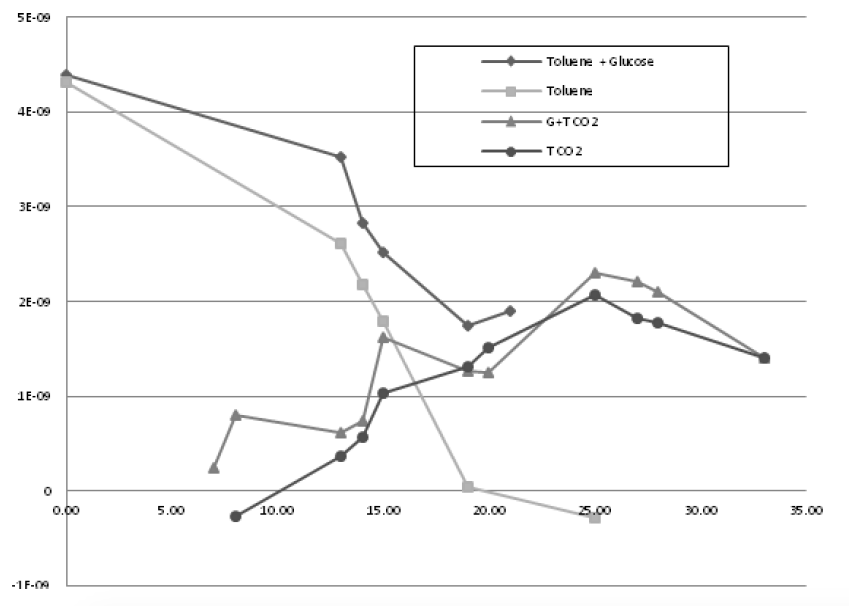
\includegraphics[width=400pt]{pics/GCresults.png}
	\caption[Toluen and CO$_2$ values for \textit{C. immunda}]
	{Toluen and CO$_2$ values for \textit{C. immunda}: Carbon equivalence [mol] of the two molecules was plotted against runtime [days]. \cite{Poyntner2014}}
	\label{GCresults}
\end{figure}

%%%% AIM OF THE THESIS %%%%%
Together all the recent studies indicate that maybe the analysis of transcriptome will answer all the question about that special fungi.
Accordingly the aim of the thesis is to exermine the way in which the transcriptomes of \textit{Cladophilaphora immunda} can be determined and identify which genes are transcribed under different conditions. The major issue is to determine the pathways that allow \textit{C. immunda} to use toluene as carbon source.\\ 
The transcriptome data were obtained with RNA-seq performed by Ion Torrent technology coupled with the Ion Proton sequencer (Life Technologies, Carlsbad, CA). \cite{BarbaraBlasi2015}
\vfill
\section{RNA-seq}
The powerful technology RNA-seq and the analysis of transcriptomes, to know which gene is expressed, became an important method in science. Transcriptome analysis enablies the understanding of how sets of genes work together to form metabolic, regulatory and signaling pathways within a cell. \cite{Xiong2006} \\
RNAs in total or fractioned are first converted into a library of cDNA fragments. Sequencing adaptors are added to each cDNA fragment to one or both ends. Each molecule is then sequenced in a high-throughput manner to obtain short sequences from one end (single-end sequencing) or both ends (pair-end sequencing).The reads are typically 30–400 bp, depending on the sequencing technology used. If the resulting sequence reads have been obtained, the first task of data analysis is to map the short reads from RNA-seq to the reference genome or to assemble them into contigs before aligning them to the genomic sequence to reveal transcription structure. The way of analysing transcriptomic data differs considering short reads also contain reads that span exon junctions or that contain poly(A) ends. Alignment can be also complicated for large transcriptomes as a result of matching multiple locations in the genome with a significant portion of sequence reads. \cite{Wang2010} \\
An advantage of RNA-seq from earlier methods, such as microarrays, is the high throughput of current RNA-seq platforms, the sensitivity afforded by newer technologies and the ability to discover novel transcripts, gene models and noncoding RNA species. \cite{Korpelainen2014} \\

\section{Bioinformatics methods}
The increasing use of next-generation sequencing methods is related to a large amount of produced data, which has to be analysed and interpreted. Therefore bioinformatics methods are a necessary step in analysing transcriptomes. As RNA-seq is an active field of research producing new approaches and tools at a rapid pace, many alternative programs exist for each analysis step. \cite{Korpelainen2014}

\subsection{Workflow System}
The data analysing steps were performed by different programs and tools, which may need specific data formats and external files. The multiple steps can be handled through scripting a reusable pipeline with defined inputs, outputs and parameters for each step. 

The software Snakemake was used to evolve the pipelines for genome annotation, functional annotation and enrichment analysis. Snakemake is based in Python language and can be used on a single core workingstation as well as on a cluster without modifying the workflow. 
Snakemake's option "--dag" creates the directed acyclic graph (DAG) of executed jobs. \cite{Koster2012}  
\newline
In figure \ref{fig:DAG} exemplified the DAG of the enduced Snakemake file. Jobs (i.e. the execution of a rule) are depicted as nodes, a directed edge between two jobs means that the rule underlying the second job needs the output of the job executed before as an input file. A path represents a sequence of jobs that have to be executed serially.
\begin{figure}[H]
	\centering	
	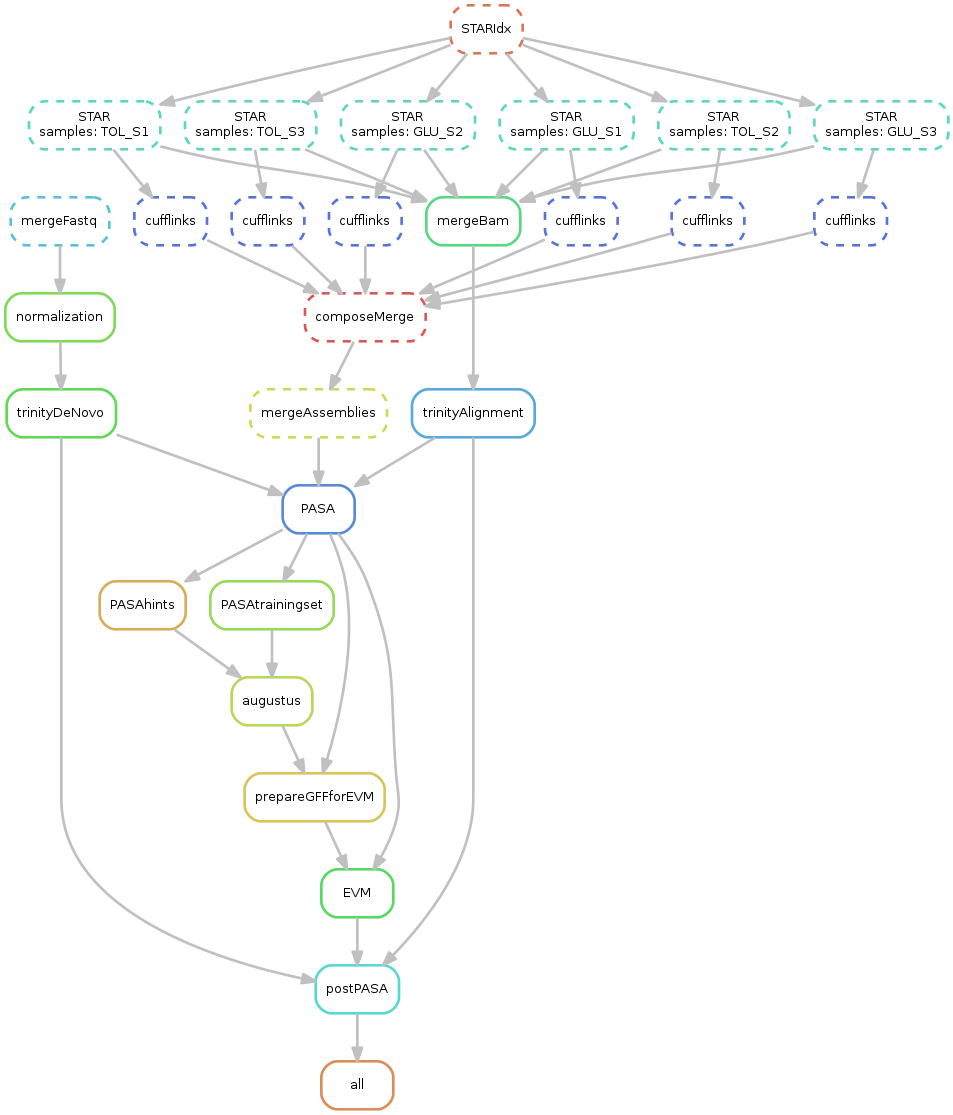
\includegraphics[width=400pt]{pics/DAG.png}
	\caption[Directed acyclic graph (DAG)]
	{Directed acyclic graph (DAG) of a Snakemakefile}
	\label{fig:DAG}
\end{figure}

\newpage
\subsection{Algorithms}
\subsubsection{Maximum Mappable Length}\label{MML}
The algortihm Maximum Mappable Length (\textit{MML}) was developed to align reads to the genome. 
The idea of \textit{MML} approach is to search a Maximum Mappable Prefix (\textit{MMP}). Given a read sequence \textit{R}, read location \textit{i} and a reference genome sequence \textit{G}, the \textit{MMP(R,i,G)} is definde as the longest substring  
\[
		 [R_{i} , R_{i+1} , ... , R_{i+MML-I} ]
\]
which matches exactly one or more substrings of G, where \textit{MML} is the maximum mappable length. 
Starting from the first base of the read the algorithm finds the \textit{MMP}. If \textit{MMP} can not be mapped contigously to the genome because of an splice junction, this first seed will be mapped to a donor splice site. The \textit{MMP} search is repeated for the unmapped portion of the read, which will be mapped to an aceptor splice site.
The difference to other algorithmn is to align the non-contigous sequences directly to the reference genome, which accelerated the process to map. \cite{Dobin2013}
\subsubsection{Expressed Sequence Tag}\label{EST}
Expressed Sequence Tag (EST) was evolved in early days of genome assembly. First the same assemblers where used for transcriptomes, but there a fundamental differences between genome assembly and transcriptome assembly. In the genome assembly the ideal output is a linear sequence representing each genomic region, whereas in the transcriptome assembly the gene is most naturally described as a graph. \cite{Korpelainen2014}

\subsubsection{de Bruijn Graph}\label{Graph}
Each node of a de Bruijn Graph is associated with a (k -1)-mer. Two nodes A and B are connencted if there is a k-mer whose prefix is the (k -1)-mer of the node A and the suffix is (k - 1)-mer of the node B. The k-mers create edges in the Buijn graph. \cite{Korpelainen2014}

\newpage
\setcounter{chapter}{2}\setcounter{section}{0}
\chapter*{Methods}
\addcontentsline{toc}{chapter}{Methods}
\section{Growth of \textit{Cladophialophora immunda}}
For the experimental conditions, the cultivation of \textit{Cladophilaphora immunda} in glucose and toluen was chosen. \\
The \textit{Cladophialophora immunda} strain (CBS 110551) was isolated from a toluene-charged air biofilter inoculated with gasoline-polluted soil. \cite{Prenafeta-Boldu2001} \\
\textit{Cladophialophora immunda} (CBS 110551) was cultured in malt extract agarose media (2 $\%$ malt extract, 2 $\%$ D-glucose, 0.1 $\%$ bacto-peptone and 2 $\%$ agar). \\
For the RNA-seq experiments, \textit{C. immunda} was grown in liquid culture in a modified Hartmans` mineral media with 2 $\%$ glucose or 1.35 mM toluene as carbon sources. \cite{Hartmans1991} The toluene was supplied through the air of a sealed flask in a 5 $\%$ solution in dibutylphtalate. The experiments duration was 90 days (growth with toluene) and one week (growth with glucose) at the temperature of 22 $^\circ$C at 100 rpm on an orbital shaker. Both experiments were performed in 3 biological replicates. At the end of the experiments the biomass was collected by centrifugation (5000 g per 15 minutes at 4 $^\circ$C), washed with RNAse free water, frozen in liquid nitrogen and stored at -80 $^\circ$C until use. \\

\begin{table}[h]
	\centering
	\begin{tabular}{c c | c c}
		\multicolumn{2}{c|}{Solution A} & \multicolumn{2}{c}{Solution B}  \\
		\multicolumn{2}{c|}{(1 litre demineralized water)}  & \multicolumn{2}{c}{(1 litre demineralized water)} \\
		\hline
		(NH$_4$)$_2$SO$_4$ & 200 g & K$_2$HPO$_4$ & 155 g\\
		MgCl$_2$.6H$_2$O & 10 g & NaH$_2$PO$_4$.2H$_2$O & 85 g \\
		EDTA & 1 g & &  \\
		ZnSO$_4$.7H$_2$O & 0.2g & & \\
		CaCl$_2$2H$_2$O & 0.1 g & & \\
		FeSO$_4$.7H$_2$O & 0.5 g & & \\
		Na$_2$MoO$_4$.2H$_2$O & 0.02 g & &\\                                
		CuSO$_4$.5H$_2$O & 0.02 g & & \\
		CoCl$_2$.6H$_2$O & 0.04 g & & \\
		MnCl$_2$.2H$_2$O & 0.1 g & & \\                          
	\end{tabular}
	\caption{Hartmans\textquotesingle mineral media}
\end{table}

The medium (1 litre of demineralized water) is compose by: \\
Solution A: 10 mL \\
Solution B: 25 mL \\
+ 0.02 $\%$ yeast extract as nitrogen source

\section{RNA-seq library preparation}
The work in the laboratory included the extraction of total RNA from 100 mg of fungal biomass with FastRNA PRO\textsuperscript{\texttrademark} RED KIT (MP Biomedicals) according to the instructions of the manufacturer. The mRNA was isolated with the Dynabeads\textsuperscript{\textregistered} mRNA DIRECT\textsuperscript{\texttrademark} Micro Kit (Ambion by Life Technologies) and the following transcriptome library preparation was performed with the Ion Total RNA-Seq Kit v2 (Life Technologies). 
Total RNA, isolated mRNA and the final cDNA library were all qualitatively and quantitatively evaluated by mean of Agilent 2100 Bioanalyzer (Agilent Technologies, Santa Clara, CA). The RNA-seq was performed by the Ion Proton\textsuperscript{\texttrademark} sequencer (Life Technologies) with the Ion PI Chip v2 (Life Technologies). 
The average read length of the six cDNA libraries was 175 bp for all five samples. Total reads generated per sample varied between 57,611,573 and 99,965,344. 

\section{Mapping Algorithm}\label{STAR}
The first step to understanding a genome structure is through genome mapping, which is a process of identifying relative locations of genes on a chromosome. When a read is mapped to reference genome, a sequence alignment is created. \cite{Xiong2006} The input files in this case were the preprocessed reads and in addition the reference sequence. \\
%%%%%Suffix tree
\subsection{Suffix Tree}
The rapid advance of new sequencing technology expand the scale and resolution of many biological applications like quantitative analysis of transcriptome where sequence reads must be compared to a reference. There are different algorithms developed in the last few years. Some of them are based on hash tables and the others are based on suffix trees. The algorithm associates two steps, identifying exact matches and building inexact alignments supported by exact matches. Finding exact matches rely on a representation of suffix tree. 
The advantage in comparison to a hash table is that by using a tree the alignment to multiple identical copies of substring in the reference has to be done only once. Because the identical copies collapse on a single path in the tree, otherwise in a hash table index an alignment must be performed for each copy. \cite{Li2010} \\
A suffix tree is a data structure that stores all the suffixes of a string to enabling fast string matching. The time complexity of determining if a query has an exact match against a tree is linear in the length of the query, independent of the length of the reference sequence. Nonetheless a tree takes \textit{O(L$^2$)} space, where \textit{L} is the length of reference. To reduce the space a approach to achieves linear space while allowing linear time searching is used. In theory it is possible to represent a suffix tree \textit{L log$_2$L + O (L)} bits using rank-selection operations. To solve this space efficient implemantation,  an enhanced suffix array was derived that consits of a suffix array and several auxiliary arrays. A suffix array can be regarded as an implicit representation of suffix tree and has an identical time complexity to suffix tree in finding exact matches. \cite{Li2010}

%%%%%Star specific approach
\subsection{\textit{STAR} specific approach}
Mapping is computationally intensive, that is why the program \textit{STAR} was chosen. \textit{STAR} (Spliced Transcripts Alignment to a Reference) is a spliced alignment program which runs very fast. The benefits of \textit{STAR} are largely based on the "maximum mappable length" approach described in \ref{MML}. \textit{STAR} splits a read and find the best portion that can be mapped for each piece. Then it maps the remaining portion, which can be far away in the case of a splice junction. The maximum mappable seed search looks for exact matches and uses the genome in the form of uncompressed suffix arrays. The second step of \textit{STAR} stitches the seeds together within a given genomic window and allows mismatches, indels and splice junctions. The seeds from read pairs are handled concurrently at this step in order to increas sensitivity. \cite{Dobin2013, Korpelainen2014}

\section{Count Algorithm}\label{featurecount}
 %%FEATURE COUNTS
Read mapping results have to be summarized in terms of read coverage for genomic features of interest. Read counts are required for statistical methods like differential expression analysis.The approach of counting the number of mapped reads to annotation was accomplished by the program \textit{featureCounts}. \\
\textit{featureCounts} performs precise read assignment by comparing mapping location of every base in the read or fragment with the genomic region spanned by each feature. It takes account of any gaps like insertions, deletions, exon–exon junctions or fusions) that are found in the read. 
The input for \textit{featureCounts} consits of aligned reads in Sequence Alignment/Map (sam) or Binary Alignment/Map (bam) format and a list of genomic features in general feature format (gff). The read alignment and the feature annotation should correspond to the same reference genome, which is a set of reference sequences representing chromosomes or contigs. \textit{featureCounts} supports strand-specific read counting with the option "-s". 
\begin{figure}[ht]
	\centering	
	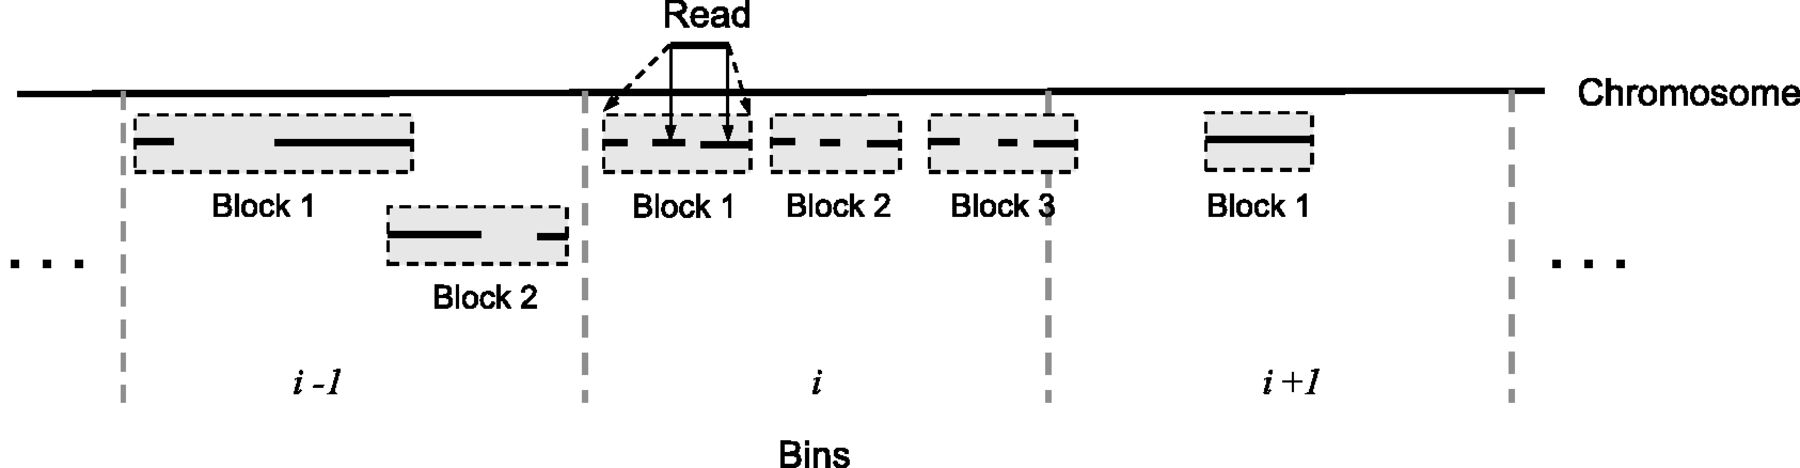
\includegraphics[width=400pt]{pics/featurecounts}
	\caption[Approach of software \textit{featureCounts}]
	{Approach of \textit{featureCounts}: genome bins and feature blocks \cite{Liao2014} }
	\label{fig:featurecounts}
\end{figure}

The algorithm is starting to generate a hash table for the reference sequence names. This enables that the reference sequence names are found to match in the input of sam/bam-files and gff-annotation quickly. Next the features in each reference sequence are sorted by their start position and a two-level hierarchy is created. Each chromosome is divided into non-overlapping 128kb bins. Features are assigned to bins according to their start postions and grouped into blocks within each bin. The query read is compared first with genomics bins, then with feature blocks within any overlapping bins and then with features in any overlapping blocks. This approach is shown in the illustration \ref{fig:featurecounts}. \cite{Liao2014}

\section{Differential Expression Algorithm}
%%LIMMA
Differential expression analysis refers to identification of genes or type of genomic features such as transcripts or exons, that are expressed in significantly different quantities in distinct groups of samples. In this study two sets of biological conditons, growth on toluene vs. growth on glucose, was compared by R/BioConductor packages \textit{limma}.\\
The first step of differential analysis is achieved by mapping RNA-seq data with \textit{STAR} (\ref{STAR}). The data input to \textit{limma} should be counts such as reads-per-kilobase-per-million (RPKM) produced by \textit{featureCounts} (\ref{featurecount}). \textit{Limma} was then used to implement differential expression. \\
The software is based on the concept of linear models with the idea to model the expression of each gene as a linear combination of some different explanatory factors. For the experiment on \textit{C. immunda} the linear model for each gene assembled by the measured gene expression (\textit{y}) is equal to the intercept (\textit{a}) representing the average expression level of the gene when the factor (\textit{condition}) is in its reference state plus the error term (\textit{e}): 
\[y = a + b * condition + e\]
A generalized linear model (GLM) is a more flexible version of a standard linear model that allows the distribution of the response variable to be different from the normal distribution used in standard linear regression. GLM assume that the read counts are distributed according to the negative binominal distribution. 
Accordingly the linear model should be written in matrix form, where the expression level (\textit{y}) is equal to experimental factor (\textit{X}) multiplied by the vector of parameters to be estimated from the data ($\beta$) plus the error term ($\varepsilon$):
\[ \mathrm{ y = X * \beta + \varepsilon}\]
Hence a contrast matrix has to be set up that describes which comparisons wants to be done. The adavantages of \textit{limma} is that it can account for more than one varying experimental factor using a generalized linear modeling framework, it is very fast and memory-intensive. \cite{Ritchie2015}

\section{Enrichment Approach}
Trough Enrichment Analysis a list of over-represented molecular funtions, biological processes and cell locations, that can then be used to test whether genes are regulating biochemical or cellular pathway, is provided. Enrichment analysis is a necessary step after data analysis for more detailed annotations about differentially expressed genes, so that a biological meaning can be postulated. \\ 
Functional annotation elements are identified with R-packages Gene Set Enrichment Analysis (GSEA) \cite{Subramanian2005} and Gene Ontology (GO) and the metabolic pathways by Kyoto Encyclopedia of Genes and Genomes (KEGG). 
A custom script was used to summarize the list of significantly overrepresented GO terms and data are graphically represented with R. \\


wird mit results ergänzt
.... \\
Funtional Annotation: 
BLAST
INTERPROSCAN
CAZY
MEROPS
TCDB (Transproter Classification database)
DVFV
antiSmash
KOBAS (KEGG Orthology Based Annotation System)



\vfill
\section{Pipeline implementation}
%overview of the pipeline used where all paramaters and thresholds are use. this leads us than to the results. 
Six samples of reads were downloaded from the sequencer-server, three of them were the transcriptomes of \textit{Cladophialophora immunda} cultivated with glucose and the other three with toluene. \\
Before implementing the workflow system a comparison of publications, different programs and tools were done. The choice of a suitable program depended on the kind of analysis and the amount of time is required. Another important issue was the option available of the used program. \\
In the beginning the reads' origin was identified by aligning them to a reference genome with \textit{STAR}. Mapped reads were used to perform transcript assembly with the softwares \textit{Cufflinks} and\textit{Trinity Genome Guided}. \textit{Trinity} also was employed for mapping-free transcript assembly. With the produced assemblies from \textit{Cufflinks} and\textit{Trinity}, the Program to Assembly Spliced Alignments (\textit{PASA}) performed the spliced alignment mapping. \textit{PASA} assemblies were utilized to create hints for the location of introns and exons. Those hints were ingrated in a hint-based run of \textit{Augustus}. Evidence Modeler (\textit{EVM}) was used to combine weighted predictions. The last step was a annotation update implemented by \textit{PASA}, where the output of \textit{EVM} compared to \textit{PASA} alignment assemblies and generated a updated gene set. \cite{Haas2011, Steijger2013, Linde2015} \\
Figure \ref{fig:pipeline} shows the draft of the entire workflow system for genome annotation with transcriptomic data. The inputs are the transcriptomes from RNA-Seq in bam-format, the genome in fasta-format and the \textit{deNovo} annotation data in gff3-format. After runs of the different steps the output is an annotation file in gff3-format.

\begin{figure}[H]
	\centering	
	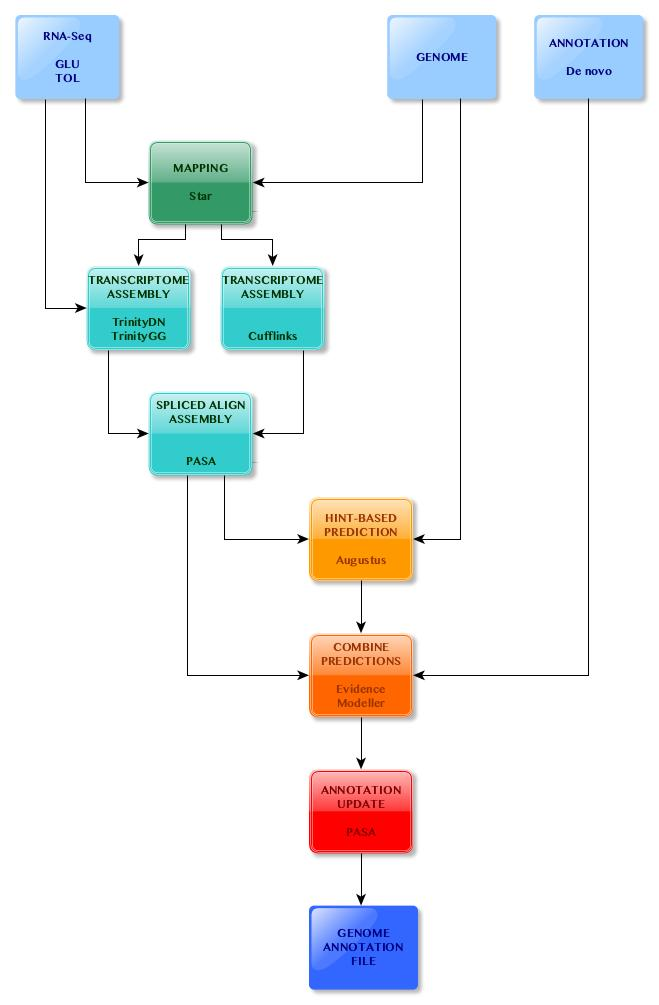
\includegraphics[width=360pt]{pics/pipeline}
	\caption[Genome Annotation Workflow]
	{Genome annotation workflow system}
	\label{fig:pipeline}
\end{figure}

%%%% Overview
\subsection*{Mapping}
\subsubsection*{\textit{STAR}}
The execution of \textit{STAR} allocated in two parts, building a reference index and mapping. Before running \textit{STAR} mapping it was obtained a reference index of the genome. Mapping of the reads was executed without the soft clip aligning at reference ends. The mapped reads needed to be sorted by \textit{Samtools}.

\subsection*{Transcriptome Assembly}
The goal of RNA-seq assembly is to reconstruct full-length transcripts based on sequenced reads. Transcript assembly answers the questions about exon regions and splice site. Several transcripts may overlap at different regions or there may be multiple copies of the same transcript. \\
There are two ways of performing transcriptome assembly. If there is a reference genome, it can be realised to guide the assembly, where the assembly task consits of solving which mapped reads correspond to which transcript. The second possibilty is to perform \textit{deNovo} assembly. \cite{Korpelainen2014} 

\subsubsection*{\textit{Cufflinks}}
The software packages \textit{Cufflinks} can be used for \textit{ab intio} reconstruction. The program within in this packages \textit{Cufflinks} assembles transcriptomes from RNA-Seq data. \textit{Cufflinks} reports the smallest possible set of isoforms. The program \textit{Cuffmerge} was used to merge the multiple assembled transcriptomes into a master transcriptome. \cite{Trapnell2010} \\
The rule \textit{Cufflinks} was implemented with the following option and values: the maximum intron length (2000) and the minimum intron length (30), the maximum number of fragment a locus may have before skipped (10000) and the library-type ff-firststrand.

\subsubsection*{\textit{Trinity}}
\textit{Trinity} consits of three seperate programs: \textit{Inchworm}, which construct initial contigs, \textit{Chrysalis} which clusters the contigs produced by \textit{Inchworm} and creates a de Bruijn Graph (\ref{Graph}) for each locus and \textit{Butterfly}, which extracts the isoforms within each de Bruijn Graph. The k-mers is fixed to be 25 in the version 2.0.2.
\textit{Jellyfish} is the software, which calculates the k-mers and therefore maximum memory has to be defined. \cite{Grabherr2013} \\
\textit{Trinity} was executed genome-guided and \textit{deNovo}. For genome-guided \textit{Trinity} the mapped reads in bam-format and for the \textit{deNovo} approach the raw reads in fastq-format were used. In both the option for strand-specific RNA-Seq read orientation for single end forward was required. 

\subsubsection*{\textit{PASA}}
Program to Assembly Spliced Alignments (\textit{PASA}) annotates protein-coding genes and alternatively splicing isoforms automatically. The goal of \textit{PASA} is to find for each alignment the largest assembly, which is used to create gene models or to modify existing gene models. \cite{Haas2003}
Further reconstructed assemblies are the input into \textit{PASA} tool. Then \textit{PASA} aligns these newly assembled transcripts to the genome using the software \textit{GMAP}. Next \textit{PASA} filters invalid alignments and those transcripts more likely resulting as artifacts of the RNA-seq assembly process and reconstructs more complete transcripts using its alignment assembly algorithm. \cite{Haas2011} \\
The recontructed inputs for the \textit{PASA} run were \textit{Trinity deNovo} assemblies, \textit{Trinity genome-guided} assemblies and \textit{Cufflinks} transcript structures. 

\subsection*{Gene Prediction}
\subsubsection{\textit{Augustus}}
\textit{Augustus} is an \textit{ab intio} gene predictor, where only a genomic sequence is needed as input information. In addition it is possible to use hints of various information. For the prediction \textit{Augustus} combines genomic sequence alignments and alignments of expressed sequenced tags (EST), described in \ref{EST}. The model underlying the program is generalized hidden Markov model (GHMM). HMMs and GHMMs for gene prediction define a probabilty for each pair ($\mathrm{\varphi}$,s) of a sequence (s) and a gene structure ($\mathrm{\varphi}$). Before starting the program \textit{Augustus} it is necessary to train the model. \cite{Stanke2006} \\
The trainingset was created from \textit{PASA} assemblies by executed the program "pasa\_asmbls\_to\_training\_set.dbi" included in \textit{PASA} package. For the additional file of hints the location of introns were filtered from \textit{PASA} assemblies. Subsequently \textit{Augustus} was started and after more than 24 hours, the output was a complete gene prediction in ggf-format. 

\subsubsection{\textit{Evidence Modeler}}
The Evidence Modeler (\textit{EVM}) is an automated eukaryotic gene structure annotation tool. \textit{EVM} reports eukaryotic gene structures by using weighted evidence combining technique. The evidence utilized by \textit{EVM} corresponds to \textit{ab initio} gene predictions and transcript alignment. \cite{Haas2008} \\
The assembly of \textit{PASA} (weight = 10), the \textit{Augustus} prediction (weight = 5) and the \textit{deNovo} Annotation (weight = 1) were combined by \textit{EVM}.

\subsubsection{\textit{Pasa Annotaion Update}}
Again Program to Assembly Spliced Alignments (\textit{PASA}) was used to update the \textit{EVM} consensus prediction by adding UTR annotations and models for alternatively spliced isoforms.


%%%%%%% RESULTS %%%%%%
\newpage
\setcounter{chapter}{3}\setcounter{section}{0}
\chapter*{Results}
\addcontentsline{toc}{chapter}{Results}
The computational results presented have been achieved in part using the Vienna Scientific Cluster (VSC). \\
%Presentation of raw results
Raw results 


\section{Up and Down regulated genes}

\section{Corresponding functional enrichment}

\section{Special Pathways}
%Toluen Pathway 

%%%%%% Melanin might be if interest



\newpage
\setcounter{chapter}{4}\setcounter{section}{0}
\chapter*{Discussion}
\addcontentsline{toc}{chapter}{Discussion}
text
\newpage
\chapter*{Conclusion}
\addcontentsline{toc}{chapter}{Conclusion}
text
\newpage
%\bibliography{/Users/christina/Documents/Bibtex/Masterthesis}
\bibliography{bib/Masterthesis}
\addcontentsline{toc}{chapter}{Bibliography}
\newpage
\listoffigures
\addcontentsline{toc}{chapter}{List of Figures}
\newpage
\listoftables
\addcontentsline{toc}{chapter}{List of Tables}

\end{document}